\section{Implementing Veritesting for Java}
In order to implement veritesting for SPF, we are leveraging existing tools and framework features within SPF.  The trickiest implementation aspects involve determining the bounds of static code regions over Java bytecodes and the mechanism for switching from ``standard'' symbolic execution using the SPF {\em SymbolicListener} class to one that can evaluate these multi-path code regions. We briefly describe our prototype implementations for these aspects.
%
\subsection{Soot-based analysis for veritesting}
%
Veritesting requires static construction of
predicates of a multi-path region which represent changes to the path expression of the dynamic
symbolic executor.
%
It also requires construction of a control-flow graph of method bodies
from Java bytecode and finding exit points of the region, which in turn
requires creation of a control-flow graph of the region.
%
Implementing veritesting is made simpler by using a static single
assignment~(SSA)~\cite{ssa} representation of the multi-path region.
%
Using an SSA form allows us to use the $\phi$-expressions created by the
SSA form and translate them into points at the end of the veritesting
region where updates to system state along different paths in the region
can be merged.
%
Soot~\cite{soot} is a static analysis framework for Java programs that
has both these features, with
ExceptionalUnitGraph~\cite{exceptionalunitgraph} and the Shimple
IR~\cite{shimple}.
%
For simple regions with only one exit point, like the one presented in Listing~\ref{lst:v_ex}, we
were able to use Soot to automate static construction of the predicate representing
an update to the expression.
%
For doing this, we used nodes with more than one successor as the
starting point, found the immediate post-dominator of the starting
point, and traversed the control-flow graph on all sides of such branches.
%
During such a traversal, we constructed predicates representing the
multi-path region, similar to the ones presented in
Listing~\ref{lst:v_ex_smt2}.
%
As explained in Section~\ref{sec:exit_points}, including virtual
function invocations in the construction of our predicates amplifies the
benefits of veritesting even further.
%
We plan to automate this inclusion in the future using Soot.
%
Providing SPF with updates to be made to its symbolic store also
requires Soot to maintain stack location information for variables.
%
We plan to automate SPF\rq s symbolic store updates using Soot in the
future.
%
\subsection{Multi-path Symbolic Execution with SPF}
%
Integration of veritesting requires changing Symbolic PathFinder so that it can 
use a Soot-based analysis.
%
We present the sequence of actions SPF must take to implement veritesting in 
Figure~\ref{fig:spf_veritesting}.
%
\lstinputlisting[caption={Listing~\ref{lst:v_ex} modified to have a return statement in the three-way branch},
label={lst:v_ex_modified}, language=Java]{code_samples/VeritestingPerf_modified.java}
%
The bytecode used in Figure~\ref{fig:spf_veritesting} was obtained by compiling 
source code shown in Listing~\ref{lst:v_ex_modified}.
%
This integration assumes our prior Soot-based analyis provides SPF 
with a table that maps instruction offsets~(representing the start of a 
veritesting region) to a set containing (1) the multi-path region predicate to be 
added to the path expression as a conjunction, (2) symbolic store
updates, (3) exit points, (4) the expression to branch on to one of the exit points.
%
Using SPF\rq s listener mechanism, we add a listener~(named
\textit{SMPListener} in Figure~\ref{fig:spf_veritesting}) which listens for instructions that are starting points for a Symbolic Multi-Path~(SMP) region.
%
On finding such an instruction, \textit{SMPListener} 
(1) updates the path expression, which may involve using the symbolic stack and/or heap, 
(2) updates the symbolic stack and heap, 
(3) creates a branch~(using SPF's \textit{PCChoiceGenerator}) to 
jump to one of the exit points~(which are instructions at offsets 40 and
41 in Figure~\ref{fig:spf_veritesting}).
%
SPF will then continue plain symbolic execution.
%
Thus, veritesting causes SPF to explore fewer branches.
%
For example, SPF only explores a two-way branch in Figure~\ref{fig:spf_veritesting}.
%
\begin{figure}[]
\caption{Veritesting with Symbolic PathFinder}
\label{fig:spf_veritesting}
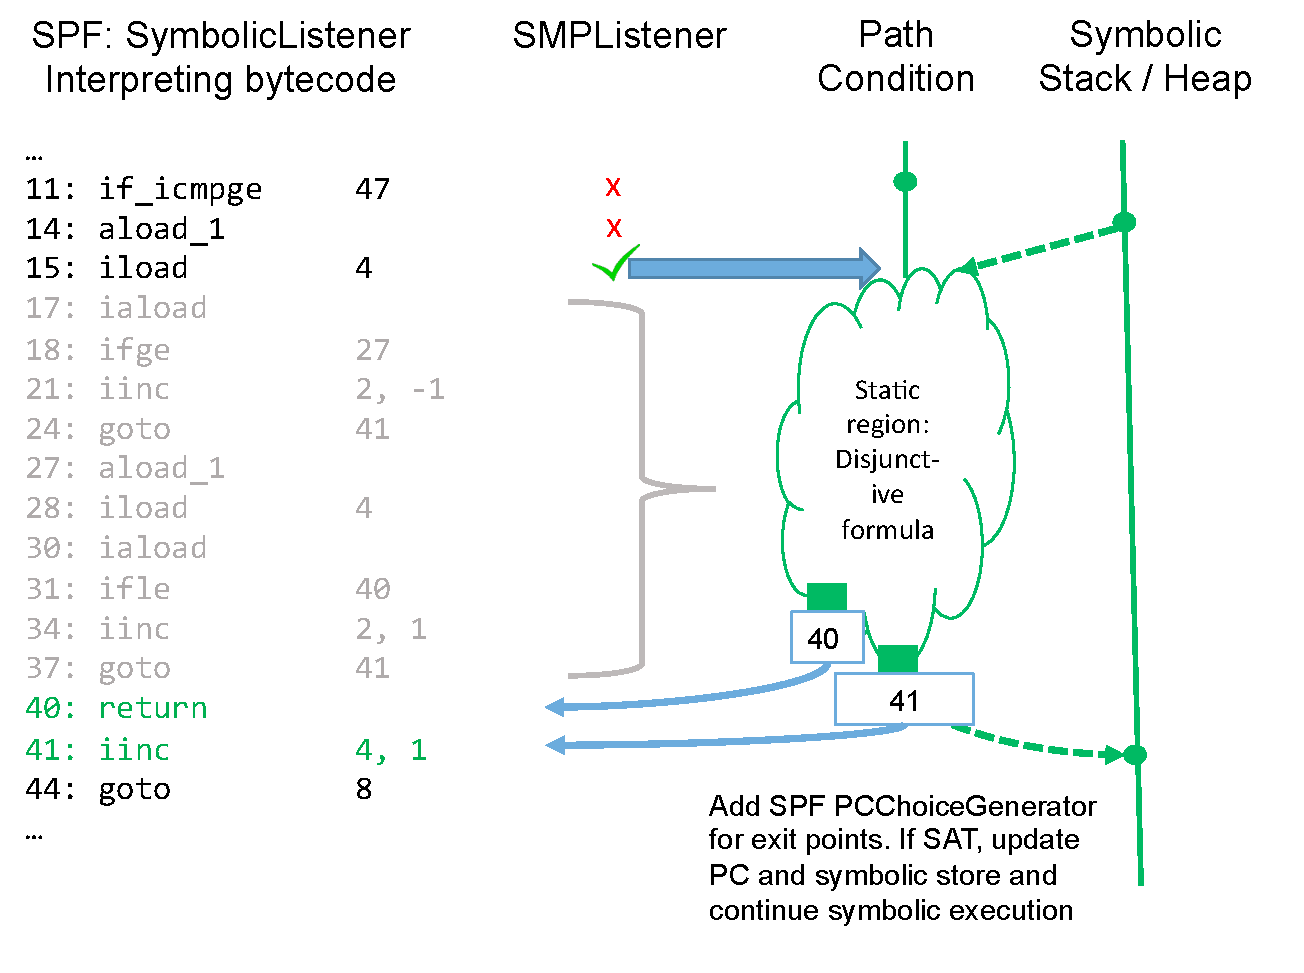
\includegraphics[width=\columnwidth]{figures/spf_veritesting}
\end{figure}
%
